\subsection{Network Economics}

A well known concept in neo-classical economy is the \textit{economies of scale}. The larger the company, the lower the price per unit of goods produced. This is known as supply-side economies of scale. Network economics can be briefly defined as \textit{``Stronger gets stronger, weaker gets weaker.''}~\cite{Shapiro1998InformationEconomy} and is interested in the opposite phenomena called \textit{demand-side economies of scale}. The key notion of demand-side economies of scale is the \textit{positive feedback} effect. When two similar technologies are on the market with a similar market share, a slight increase in popularity of one technology can create a perception that this technology is better and will win the entire market. This perception is reflected in the market, where even more consumers choose the slightly more popular technology, raising the market share and strengthening the perception... and so on in a loop, until the technology finally takes over the market. This is known as tipping and can be initiated by an small impulse (e.g. a successful marketing campaign)~\cite{Shapiro1998InformationEconomy}. The market condition over time is illustrated in Firure~\ref{fig:tipping}.

\begin{figure}[ht]
    \centering
    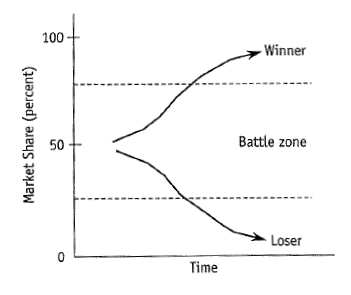
\includegraphics[width=0.6\textwidth]{00images/shapiro}
    \caption{Market during positive feedback. Taken from~\cite{Shapiro1998InformationEconomy}.}
    \label{fig:tipping}
\end{figure}

A typical example is the one of VHS vs. Betamax tapes, where there were two similar (but incompatible) products offered on the market. Minor differences (longer recording time) tipped the market towards VHS, pushing Betamax into the niche zone.

